\section{Flow: overview}
\label{sec:flow-overview}

Flow is a prototype of a multi-user ``exploration game'', in which participants navigate and interact with a virtual world rendered in a game engine using a combination of inputs: 
\begin{enumerate}
\item \textit{Indoor positioning}: participants' positions in physical space, detected by indoor positioning (person tracking), modify the virtual landscape;
\item \textit{Wearable sensing}: participants directly control orientation of the environment's virtual camera using gyroscopes connected to microcontrollers, which can be worn or carried; 
\item \textit{Mobile phone interface}: participants interact with the virtual environment through controls on their smartphone, for example to share social media images in the virtual environment.
\end{enumerate}
In addition to various types of IoT devices and the game engine, the system on which Flow is built also includes an \textit{authentication server} (AS) that performs local trust management.

\begin{figure}[!t]
\centering
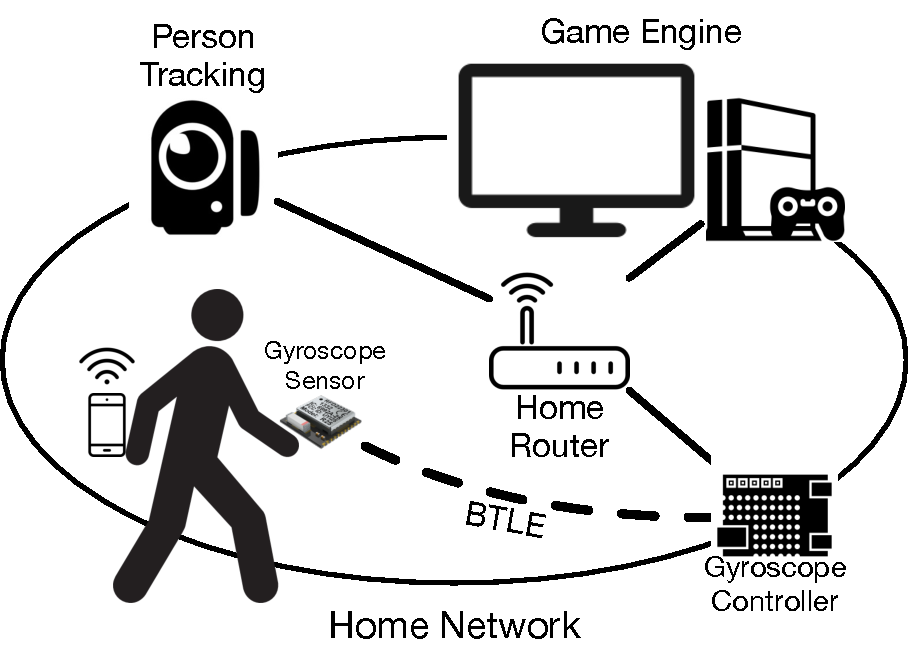
\includegraphics[width=0.9\columnwidth]{flow-home-deployment.pdf}
\caption{Typical deployment of the Flow home entertainment experience.}
\label{fig:flow-deployment}
\end{figure}

Figure~\ref{fig:flow-deployment} shows a typical deployment scenario of Flow in a home network.
NDN interconnectivity between different components is supported over Ethernet and Wi-Fi, through the home Wi-Fi router in a hub-and-spoke topology.
Sensor devices with limited networking capability (e.g., the gyroscope in Fig.~\ref{fig:flow-deployment}) may be bridged via a helper device.
We assume all devices can reach each other over NDN, which is trivial in a hub-and-spoke topology.

While analyzing the components of Flow, we re-examined the building blocks described in Section IV of \cite{ndn-iot}, and found their patterns common in the implementation of Flow application. 
Thus we separate the common functionality, including naming, bootstrap, discovery, and application level pub/sub, from the application and implemented them in a framework called Named Data Networking of Things Framework (NDN-IoT), which we believe may facilitate the development of traditional home automation systems and many other IoT applications. 
